\chapter{Introduction}
\label{Introduction}

\begin{flushright}{\slshape    
The real problems going forward are not with any single device, \\
but in the potential complexity of the larger ecosystem of \\
technologies that we function in. [...] It's about the society \\
of appliances and how they work today which is the new frontier.} \\ \medskip
    --- Bill Buxton \cite{Buxton2010}, HCI researcher and designer
\end{flushright}

\marginpar{Parts of this chapter appear in \cite{Niezen2010} and \cite{Niezen2011}.}

%-- 20-liner
When trying to share music or photos between your mobile phone and that of a friend, making the connection between the two devices is not always straightforward. You need to select the appropriate communication technology and identify the target device from a list of possible options. Manufacturers often only allow sharing between devices that form part of their own ecosystem, where devices from other manufacturers may be incompatible with this ecosystem. In the future there could be hundreds of devices in your immediate surroundings, and these devices, created by different manufacturers, will need to work with another.

What if we want to share more than just media, or want to use one device to control another? As an example, imagine connecting a sleep monitor to the lamp on your bedside table, helping you to wake up at the right time in your sleep cycle. This thesis focuses on ways to create meaningful connections between devices, based on the functionality of the devices. We develop techniques for designers and developers to describe the capabilities of devices, such that the content and functionality can be shared with other devices. We also make use of different types of feedback to indicate what the possibilities for interaction are, as well as making the events that occur within this system of networked objects more transparent.

%---
\marginpar{Mark Weiser \cite{Weiser1991} coined the term ubiquitous computing, sometimes seen in its shortened form as ``ubicomp''.}
Key to realising the vision of ubiquitous computing \cite{Weiser1991} is ``serendipitous interoperability'', where devices which were not necessarily designed to work together should be able to discover each other's functionality and be able to make use of it \cite{Owl2004}. Future ubiquitous computing scenarios involve hundreds of devices, appearing and disappearing as their owners carry them from one room or building to another. Therefore, anticipating all the different types of devices and usage scenarios a priori is an unmanageable task. 

Next to serendipitous interoperability, another enabling strategy of ubiquitous computing is to make technologies --- as from a user's perspective they are still dealing with technologies --- disappear, and ``weave themselves into the fabric of everyday life until they are indistinguishable from it'' \cite{Weiser1991}. To reach this goal, self-configuration of the various devices and technologies in ubiquitous computing environments is essential. Whether automated and initiated by context-aware entities, or initiated by users by connecting the devices to one another, the actual configuration of the various components at a lower level should happen automatically.

\section{Background}

\subsection{Multi-device user interaction}

As computers disappear into the environment, we will need new kinds of human-computer interactions to deal with the peculiarities of these smart environments, which include invisible devices, implicit interaction, and distinguishing between physical and digital interactions \cite{Ye2007}. In the conventional \ac{GUI} genre, designers have typically developed prepackaged solutions for a predetermined interaction space, forcing users to adapt to their specific interaction protocols and sequences. In ubiquitous computing environments, the interaction space is unpredictable and emerges opportunistically \cite{Coutaz2005a}. There is the risk of creating a mismatch between the system's model of interaction and the user's mental model of the system. In these conditions, new interaction techniques must be devised to help users to construct helpful mental models, in order to minimise system and user model mismatches. These interaction techniques should also match the context of use that is dynamic and unpredictable. 

% A related issue is how ubiquitous computing differs from the sequential nature of traditional \ac{GUI} interaction. The single point of control that is usually available in such interfaces naturally leads to a sequential organisation of interaction. One step inevitably leads to the next; as an example, consider a dialog box that refuses to let you do anything else until you click either \texttt{OK} or \texttt{Cancel}. When we interact with a smart environment, it is not only the parallel nature of the interaction with the physical world that is different, but also \emph{the many different ways that we might map our tasks onto the features of the environment} \cite{Dourish2004}. Another difference is that these are not necessarily single-user interactions, but multiple users interacting in the same smart environment at the same time.

If we are able to connect smart devices to one another effortlessly, it becomes possible to support high-level services, that would usually involve multiple steps on multiple devices \cite{Rich2009}. From a user's point of view, streaming music from a mobile device to a home entertainment system is a single high-level task. In practice there are multiple steps involved, and if the devices involved are from different manufacturers, the user needs to learn the operational details of each device interface in order to perform the task. From a technical perspective \ac{UPnP} with its device control protocols \cite{uPnPDCP} is not considered an adequate solution, because it only provides static device description documents and covers a very limited number of use cases. %From a user perspective \ac{UPnP}

At home the average person interacts with many devices during the course of a day. Sometimes these devices are used by more than one person, or one device may be used as an interface to another. As these devices are manufactured by different companies, there exist many different user interfaces that must be studied before they can be used. There might even be more than one way to interact with a single device. For example, to turn down the volume on a home entertainment system, either a remote control or a volume dial on the entertainment system itself may be used. It is expected that in future, more generic tools will be used to discover, configure, connect and control all the devices in the environment \cite{Newman2002}. 

\subsection{Configuring connections between devices}

In a world where we are potentially surrounded by a multitude of devices, allowing for the arbitrary ad hoc interconnection of devices, and the sharing of information between these devices, is difficult. It is unreasonable to expect that a device will have prior knowledge of all the different ways it can interact with surrounding devices. The number of possibilities are too large, and anticipating the potential number of interactions is infeasible. If we could add meaning to the interactions and interconnections in such a way that it is machine-readable, semantic web technologies could be used to infer additional properties about the existing entities. This could fill the gaps between that which is described in terms of device capabilities, and that which is possible in terms of combined functionality. The user is still the final arbiter in deciding what the device does, but the device should be capable of communicating the possibilities based on what was inferred from its environment. 

Besides the technological challenges, there also lies a challenge ahead for designing user interactions with these ecosystems of interconnected devices. When moving away from interaction with a single device towards interactions with systems of devices, designers need to communicate the relationships between the devices, and the larger system they are part of. Additionally, designers need to find ways to communicate the action possibilities of new, ``emergent functionalities'' \cite{Frens2009}, that emerge when devices are being interconnected. 

An important problem that arises when designing for these systems of interactive objects is their highly interactive and dynamic nature \cite{Frens2009}. The inherent ever-changing nature of these systems and the severely limited overview of the ecosystem in its entirety is one of the most important challenges a designer faces when designing for such systems. Additionally, such a system comprises many different ``nodes'' that the designer, at the time of designing has no control over. Yet, when designing and adding new nodes to the system, making them interoperable is crucial for success. 

According to Newman et al. \cite{Newman2002}, the following should be communicated to a user attempting to interact with and establish connections between devices:
\begin{itemize}
\item What devices and services are available
\item Capabilities of the devices and services
\item Relationships between each another and the environment
\item Predictions of likely outcomes from interaction
\end{itemize}

The information presented to the user should be filtered dynamically, based on the user's context. This context includes for example the user's location, interaction history, and current tasks. A smart object is able to sense the context of its surroundings, make use of this context and other information to proactively interact with users and other smart objects, and self-organise into groups with other devices \cite{Sabou2010}. This context information should be represented in such a way that is understood by all the entities in the system. 

%When people think of systems that try to infer what they are doing from their actions, they inevitably think of Clippy, Microsoft's Office Assistant, that tried to offer help based on a user's actions.

The background described in this section provides for interesting design challenges and research questions that can be asked. In the following section we will first discuss the context of the work described in this thesis, followed by the research questions that were addressed.







\section{Context of the work and research questions}

The work described in this thesis was completed as part of a European research project called \ac{SOFIA}\footnote{http://www.sofia-project.eu/}. Some of the design choices were guided by collaboration with partners in the \ac{SOFIA} project. We worked with the project partners to elicit requirements and expose ourselves to other application areas, in order to gain a more holistic view of the problem.


\subsection{The SOFIA project}\label{sofia}

\ac{SOFIA} is an European research project within the ARTEMIS framework that attempts to make information in the physical world available for smart services --- connecting the physical world with the information world. The goal is to enable cross-industry interoperability and to create new user interaction and interface concepts, to enable users to benefit from smart environments. The centre of the software platform developed within \ac{SOFIA} is a common, semantic-oriented store of information and device capabilities called a \ac{SIB}. Various virtual and physical smart objects, termed \acp{KP}, interact with one another through the \ac{SIB}. The goal is that devices will be able to interact on a semantic level, utilising (potentially different) existing underlying services.

%thimbleby
\label{sofiatuple}
The \ac{SOFIA} software platform is based on the ideas of space-based computing, where near linear scalability can be achieved using the tuple space paradigm. A tuple space is a repository of tuples, where a tuple is an ordered list of elements. Tuple-based computing has been introduced in parallel programming languages to implement communication between parallel processes \cite{Fensel2004}. Producers send their data as tuples to the space, and consumers read tuples from the space. This is also known as the blackboard metaphor.

Our focus within the \ac{SOFIA} project was on the user interaction aspects of devices in the smart home environment. While most of the examples in this thesis are specific to the smart home environment, the concepts are also applicable in the wider context of ubiquitous computing, for example the smart city or smart personal spaces. %We now look at the context of the work in terms of two complementary visions described in the literature: Ubiquitous computing and ambient intelligence.
We now consider the context of the work in terms of the vision of ubiquitous computing.

\subsection{Ubiquitous computing}

%Mark Weiser \cite{Weiser1991} coined the term ubiquitous computing, sometimes seen in its shortened form as ``ubicomp''. 
The vision of ubiquitous computing describes a future where electronic devices are so ubiquitous that their presence is not noticed anymore. As described earlier in this chapter, we consider the enabling technological strategies of ubiquitous computing to be serendipitous interoperability and making technologies disappear.

Chalmer and MacColl \cite{Chalmers2003} questioned the more recent assumption in ubiquitous computing research that devices should disappear into the environment, reiterating Weiser's original vision that tools for interaction should be ``literally visible, effectively invisible''. There is a difference between physical and cognitive disappearance. Where the term physical disappearance describes the trend of devices to be embedded into the environment, cognitive disappearance means that the user does not distinguish between the computer and the artefact anymore, but focuses on the function of the artefact. Devices should retain their unique characteristics, even when placed within systems of devices. Users are influenced by how they perceive devices, and we have to accept that the devices themselves are part of the user's context.

Ubiquitous computing products are a combination of hardware, software and services. It is not clear what kind of skills are required to design for this kind of environment \cite{Kuniavsky}. There is, however, a need for interaction designers and software developers to have a common vocabulary and framework when cooperating to create these products. This thesis attempts to move this idea forward, by defining common concepts that are prevalent in most ubiquitous computing environments, and establishing a framework that can be used by both designers and developers alike.

% \subsection{Ambient Intelligence}
% The Ambient Intelligence paradigm differs from that of Ubiquitous Computing in that it tries to create environments that are sensitive  to and responsive to the presence of people \cite{Aarts2004}. Devices disappear into the environment, necessitating virtual devices to support user interaction. It is expected that the devices adapt to to and even anticipate the user's needs. While our work is in principle closer to the vision of ubiquitous computing than ambient intelligence, there are some important aspects of ambient intelligence that need to be considered.
% 
% % Start of SISS2010 Conclusion
% 
% Marzano and Aarts \cite{Aarts2004} formulated the following five key technology features to define the notion of ambient intelligence:
% 
% \begin{itemize}
% \item Embedded - many networked devices are integrated into the environment.
% \item Context aware - the system can recognise the user and his/her situational context.
% \item Personalised - the system can tailor itself to meet the user's needs.
% \item Adaptive - it can change in response to the user.
% \item Anticipatory - the system anticipates the user's desires without conscious mediation.
% \end{itemize}
% 
% Personalisation refers to system adjustments made on short time scale, for example installing personalised settings. Adaptation involves adjustments made by monitoring the user over a longer period of time. For anticipation, the system needs to be able to detect behavioural patterns that occur over a very long period of time.
% 
% %We consider context awareness to be one of the most important features of a smart environment, especially when we consider a user's interaction with the smart space. Considering the parallel nature of our interaction with the physical world, any smart space will require context to help it make sense of the many different ways in which users map their tasks onto the environment.
% 
% Where the system tries to predict what the user is trying to accomplish, by being adaptive and anticipatory, we need to identify ways to give the users appropriate means to express themselves. The possibilities, available services and information that exist in the smart environment need to be communicated in a meaningful way. Only if this is done correctly will users be able to build helpful mental models of the functionality the environment has to offer, set goals and make plans on how to act. By developing novel and meaningful interaction devices, the user can then perform the necessary actions and the system can in turn try to understand the user's goals and make the match to its internal models. We see a vital role here for the theory of \emph{product semantics} \cite{Feijs2009}, the study of how artefacts acquire their meaning, where we can use its theories to define common concepts and semantics.
% 
% The ambient intelligence paradigm shows the importance of feedback in adaptive and anticipatory environments. In the thesis we describe the different kinds of feedback and feedforward that are applicable to these environments, as well as how it was implemented in a use case scenario. 


\subsection{Affordances}

In their article ``At Home with Ubiquitous Computing: Seven Challenges'', Edwards and Grinter \cite{Edwards2001} describes a scenario where a couple come downstairs in the morning intent on listening to the radio, and realise that there is no sound coming from their speakers. It turns out that the neighbours bought a new set of Bluetooth-enabled speakers which, when installed, associated themselves with the nearest sound source -- the couple's Bluetooth-enabled stereo.

The wireless nature of the speakers does away with the traditional affordances making connections between the speakers and the stereo. These affordances are explicit when physical wires are used - the connections can be observed and the range of connectivity is clear. Edwards and Grinter state that the design challenge is to provide \emph{affordances}\label{Affordances} that help users understand the technology, allowing them to control, use and debug technologies that interact with one another in the environment. 

Norman \cite{Norman1999} defined affordances as the perceived and actual properties of an object, primarily those properties that determine how an object should be used. The set of action possibilities of an object is based on its appearance, but also on the actual interaction with that object. An affordance is a relationship between an object and the person acting on the object, such that the same object might have different affordances for different individuals. The term was originally created by the psychologist J.J. Gibson to describe human perception \cite{Gibson1977}, but was extended by Norman for its application to design.

%Complex interactions between numerous interconnected computers and devices, where functionality is distributed across several devices that are spontaneously discovered and used, need to be managed \cite{Lee2006}.

% Interaction metaphors \cite{Kuniavsky} provide handles to these invisible technologies, where the metaphors are used to establish ideas about the meaning of physical affordances and potential ways to use these devices. For example, a Nintendo WiiMote is waved around much like a magic wand, so we can use ``an enchanted object'' as the interaction metaphor for the device.

\subsection{Ontologies}

The current state of ubiquitous computing is similar to that of desktop computing in the 1970s, where there is a whole range of new technologies without metaphors to communicate how they operate. The question then becomes how we then can model a device, not only in terms of its technical characteristics or capabilities, but also in terms of user interaction and feedback, where metaphors, functionality and affordances play an important role.

One possible solution to modelling devices is to make use of ontologies, a concept in computer science most often associated with the Semantic Web \cite{Berners-Lee2001}. Ontologies are formal representations of knowledge, consisting of various entities that are related to one another. They provide a shared vocabulary, which makes it easier to publish and share data. Ontologies allow us to model a domain in terms of its concepts, and the relationships between these concepts. They are also both machine-readable and human-understandable.

Ontologies are well suited to environments with a large number of devices. They have been designed to work at Web scale, they enable heterogeneous data sources to interoperate with one another, and they are based on technology standards which allow for easy and large scale adoption \cite{Sabou2010}.
 
Ontologies lend themselves well for describing the characteristics of devices, the means to access such devices, and other technical constraints and requirements that affect incorporating a device into a smart environment \cite{Owl2004}. Using an ontology also simplifies the process of integrating different device capability descriptions, as a semantic inferencing engine can be used to infer relationships between the concepts in the descriptions.


\subsection{Research questions}
\label{ResearchQuestions}
The hypothesis of this thesis is that \emph{user interaction in a smart environment can be better supported by ontological models than with existing device and service descriptions} (e.g. descriptions stored in relational databases). These ontological models define a semantic mapping between the user's behaviour and the available resources in the environment.

%Should be measurable, specify what is compared and what is being verified. Relate to existing body of knowledge. Research question should be stated in observable, measurable terms

\marginpar{``The greatest challenge to any thinker is stating the problem in a way that will allow a solution.'' -- Bertrand Russell}

The thesis aims to answer a number of research questions. In the previous section, ontologies were offered as a potential solution to solving the interoperability problem in ubiquitous environments. They are also well suited to describing user interaction in such an environment. This leads us to the first question:

\begin{question}
How can we use an ontology to model user interaction and devices in a smart environment consisting of multiple devices and multiple interactions? 
\end{question}

%thimbleby
Related work on ontologies \cite{Chen2004,Ranganathan2004,Ngo2004}, described in more detail in the next chapter, focused mainly on modelling context and basic device properties. The ontologies created as part of the work described in this thesis is not only an attempt to model device capabilities in more detail, but to our knowledge is also the first attempt to model user interaction in a smart environment. 

%This question is addressed in Chapters \ref{DeviceCapabilityModelling}, \ref{EventModelling} and \ref{OntologyEngineering}. %How can interaction events be modeled, represented and reasoned about using a ontology language?

% TODO Discuss http://en.wikipedia.org/wiki/Publish/subscribe, or change to blackboard pattern
\label{blackboard}
In the \ac{SOFIA} project, \acp{KP} communicate with a message broker using the blackboard architectural pattern, where the message broker contains a common knowledge base. This knowledge base, consisting of a triple store and an ontology, is used to share information between the various knowledge sources.

\begin{question}
How suitable is the blackboard architectural pattern for handling ontology-based ubiquitous computing environments? 
\end{question}

%lukkien
Suitability is defined in terms of user interaction, where the performance of the combination of a triple store, semantic reasoning and the blackboard architectural pattern is evaluated in terms of responsiveness.

%thimbleby
The advantage of a blackboard architecture is that it decouples reference, time and space \cite{Fensel2004}. Communicating processes do not need to explicitly know each other, i.e. reference-wise they are decoupled. The blackboard guarantees persistent storage, such that communication can be asynchronous and decoupled time-wise. As long as they have access to the same blackboard, processes can run anywhere, decoupling them space-wise. We can compare the performance of our implementation against related work on blackboard-based architectures for ubiquitous computing environments \cite{Winograd2005,Etelapera2011}. 

%Chapter \ref{SoftwareArchitecture} seeks to answer this question.

If we make use of a triple store and ontology, a semantic reasoning engine is required to perform inferencing on the knowledge base of asserted triples. If triples are frequently inserted and removed, the time required for inferencing could have an adverse effect on the responsiveness of the user interface.  

\begin{question}
How responsive is a networked user interface that is implemented on top of a system architecture with a semantic reasoning engine? 
\end{question}

%This question is addressed in Chapter \ref{Evaluation}.

Some work has been done to measure the usability of \acp{API} for developers \cite{Robillard2009}. However, we do not have a way to evaluate the usability of software frameworks and ontologies for ubiquitous computing environments from a developer point-of-view. 

\begin{question}
How can we measure the usability of ontologies and software frameworks for developers of ubiquitous computing environments? 
\end{question}
%This is explored further in Chapter \ref{Evaluation}.

Feedback is required to help the user make sense of what is happening in the environment. When we consider multiple interconnected smart objects, feedback and feedforward gets spatially distributed. 

\begin{question}
How should feedback be provided in a networked user interface consisting of multiple connected devices? 
\end{question}
%A possible solution to this problem is presented in Chapter \ref{DesignIteration3}.

%How can description logic be applied to the modelling of smart environments?

% How should the capabilities of devices in the environment be modelled in order to perform semantic mapping?
	
%How can we use semantic reasoning to infer user intention in a smart environment?

%After making inferences about the user, how should a user-adaptive system respond?

%What emergent knowledge is created through ad-hoc interactions between connected devices?

%Why is an ontological approach better than existing approaches, e.g. relational database?

%\end{itemize}

%- Describe devices based on their capabilities/attributes, and use reasoner to infer connection possibilities.
%- Multi-device user interaction
%- Abstracting low-level interaction events into higher-level actions/goals/tasks
%- Functional coupling between mobile devices
%-  
%- Information filtering based on context and current goals
%- Publish/Subscribe messaging paradigm
% - Systems that obtain user input through sensing user action, rather than through standard input devices such as the keyboard, mouse or stylus.
%- Does not cover graphical user interfaces, but interaction events

%Building a model of the user's interaction with the smart space allows us to establish a semantic mapping between user behaviour and the environment. 
%Ontological modelling may be used to create an interaction model of a user's interaction with the smart space, including the user's profile, preferences, goals and intentions. We may use the interaction model to map the user's tasks or goals onto the devices available in the smart space.  Devices should focus on supporting people's stated intentions, desires and needs, rather than trying to anticipate them \cite{Kuniavsky}.

\section{Methodology}

\begin{figure}
\centering
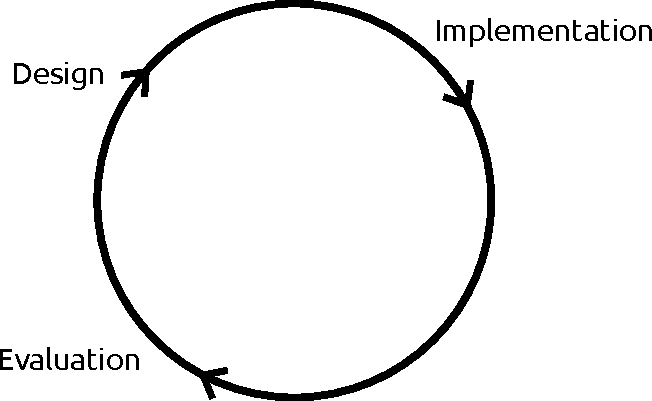
\includegraphics[width=250px]{methodology}
\caption{Iterative design methodology}
\label{methodology}
\end{figure}

%there should be a separate section "approach" or "methodology", to present the methods and the process of the investigation, and in answering the research questions.

An iterative design methodology \cite{Larman2003} was followed for the work described in this thesis. This cyclic process, shown Figure \ref{methodology}, consists of three steps -- design, implementation and evaluation -- where the results of the previous iteration are used as input for the next iteration. Iterative design is commonly used in the development of human-computer interfaces, but applies to many fields, including industrial design and software engineering.

%thimbleby
The research described in this thesis can be aligned to the triangulation framework of Mackay and Fayard \cite{Mackay1997}, as shown in Figure \ref{roadmap}. This framework integrates scientific and design models, by combining the deductive and inductive approaches with the design approach. With the deductive approach, research originates from theory, whereas with the inductive approach the research originates from observations. With the design approach, designers and engineers use guidelines and requirements as input to iterative prototypes used to construct a final product.

The framework shows how the design iterations are related to the constructed theories and models, as well as the evaluations and observations. The framework provides a roadmap of the work described in this thesis, where the relevant chapters are indicated in the figure.
  
\begin{figure}
\centerline{
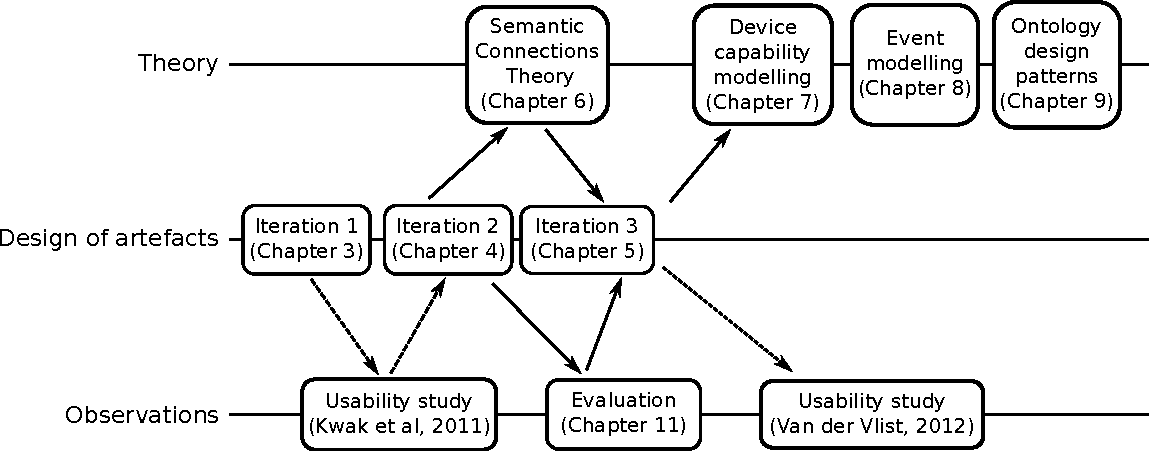
\includegraphics[width=450px]{Roadmap}}
\caption{The research approach used in the thesis}
\label{roadmap}
\end{figure}


\section{Outline of the thesis}

In the remainder of Part A the related work, including relevant research projects, is discussed. Existing state-of-the-art ontologies for ubiquitous computing environments and context-aware systems are described, followed by a description of the various interaction models, task models and semantic models that were used as basis for our own interaction model. 

An iterative approach was followed during the design process. Part B describes the three design iterations, detailing the requirements, design, implementation and evaluation processes. A theory of semantic connections is introduced, based on the output from the design iterations, that focuses on the meaning of the connections between the different entities in a smart environment. It is intended to enable interaction designers and developers to create interoperable smart objects, providing them with a common vocabulary and framework. The \ac{SOFIA} software architecture was taken as a departure point during each of the design iterations described in Part B. The various extensions and changes to the reference architecture are described in more detail in each design iteration description. 

From the work done, concepts and techniques that can be applied to ubiquitous computing in general were discovered. These concepts and techniques were extracted from the design iterations and are discussed in more detail in Part C, to exist independently of the design iterations. Our approach to modelling the interaction capabilities of smart objects is described, which builds on earlier ontologies for context-aware systems. Another contribution of this thesis is in the way interaction events are modelled, utilising existing event modelling techniques to describe user interaction in smart environments. Ontology design patterns that were identified and used during the course of the design are documented. A proposed software architecture to be used in future ubiquitous computing scenarios, based on the work done within \ac{SOFIA}, is described. This is followed by an evaluation of the work, which includes a performance evaluation and usability analysis. 



%In this thesis, the various models and technologies that may be combined to allow for semantic interaction in smart environments are investigated. 
%  We also consider whether the blackboard architectural pattern, used by SOFIA to enable a smart space-based computing environment, may be combined with runtime task models and the Belief-Desire-Intention (BDI) model, to result in a usable software architecture for pervasive computing.



